\documentclass{beamer}
% \usepackage{beamerthemesplit} // Activate for custom appearance
\usepackage{beamerthemesintef} % comment this line + everything with '%%%' if you don't have the theme installed

\titlebackground*{assets/background} %%%
\title{MPC-PiNNs technique applied to Quadrotors}
\subtitle{Elective in Robotics [UAV] Course Project}
\course{Master's Degree in Artificial Intelligence and Robotics} %%%
\author{{Authors}} %%%

\IDnumber{matricole} %%%
\date{Academic Year 2024/2025}

\begin{document}
\maketitle
\section{Introduction}
\begin{frame}{Neural Model Predictive Control (NMPC)}
    In this work we have tried to combine Model Predictive Control along with PiNNs to trajectory tracking problem applied to quadrotors. We have used the Unicycle robot as simple test case for our experiments.
\end{frame}
\section{Robot Models}

\begin{frame}{Quadorotor}
    \begin{columns}[T] % Align columns at the top
        % Left Column: Text
        \begin{column}{0.45\textwidth}
            \vspace{0.7cm}
            Since we have used the Crazyflie robot as reference, we have used a first order model because the robot takes as control inputs RPY desired poses rather than torques. This means that the output of the MPC gives us the RPY desired poses while the ODE model gives us the velocity commands.
        \end{column}
        
        % Right Column: Equation
        \begin{column}{0.50\textwidth}
            \vspace{-1.0cm}
            \begin{align}
                \begin{cases}
                    \dot{x} = v_{x}, \\
                    \dot{y} = v_{y}, \\
                    \dot{z} = v_{z}, \\[1ex]
                    \dot{v}_{x} = -\Bigl(\cos\psi\, \sin\theta\, \cos\phi + \sin\psi\, \sin\phi\Bigr)\frac{T}{m}, \\
                    \dot{v}_{y} = -\Bigl(\sin\psi\, \sin\theta\, \cos\phi - \cos\psi\, \sin\phi\Bigr)\frac{T}{m}, \\
                    \dot{v}_{z} = -\Bigl(\cos\theta\, \cos\phi\Bigr)\dfrac{T}{m} + g, \\
                    \dot{\phi} = ({\phi_{c} - \phi})/{\tau} \\
                    \dot{\theta} = ({\theta_{c} - \theta})/{\tau} \\
                    \dot{\psi} = ({\psi_{c} - \psi})/{\tau} 
                \end{cases}
            \end{align}
        \end{column}
    \end{columns}
\end{frame}

\section{Model Predictive Control}
\begin{frame}{Model Predictive Control}
    This approach leads to good result for both the drone and unicycle models.
    \begin{align}
        \min_{u(0), u(1), \dots, u(N-1)} \quad & \sum_{k=0}^{N-1} \ell(x(k), u(k)) + \ell_f(x(N)) \\
        \text{s.t.} \quad & x(k+1) = f(x(k), u(k)), \quad k = 0, \dots, N-1, \\
        & x(k) \in \mathcal{X}, \quad u(k) \in \mathcal{U}, \quad k = 0, \dots, N-1, \\
        & x(0) = x_{\text{0}}
    \end{align}
\end{frame}
\begin{frame}{Crazy-MPC}
    Our objective is to minimize at each step the error with respect to the reference
    trajectory, while also maintaining the module of the input actions as low as possible.
    \begin{itemize}
        \item The \textbf{decision variables} are $(\phi_{c},\theta_{c},\psi_{c}, T)$ and the state of the robot
        \item The \textbf{constraints} are related only to the decision variables
        \item The cost function minimizes the distance between the state of the quadrotor and the reference trajectory at time $t_{k}$
    \end{itemize}
\end{frame}

\section{Neural Network}
\begin{frame}{Simple MLP}
    \begin{columns}[T] % align columns at the top
        \begin{column}{0.50\textwidth}
            The architecture is characterized by two hidden layers of 128 neurons and takes as input the current state and the action that I want to apply.
            \vspace{1ex}
            \begin{align}
                \dot{x} &= f_{\theta}(x,u) \\
                loss &= \frac{1}{k}\sum_{i=t}^{t+k} (\bar{s}_i - s_i)^2
            \end{align}
            The loss is computed as the MSE between the neural and the nominal evolutions of the state.
        \end{column}
        \begin{column}{0.4\textwidth}
            \centering
            % First image on top
            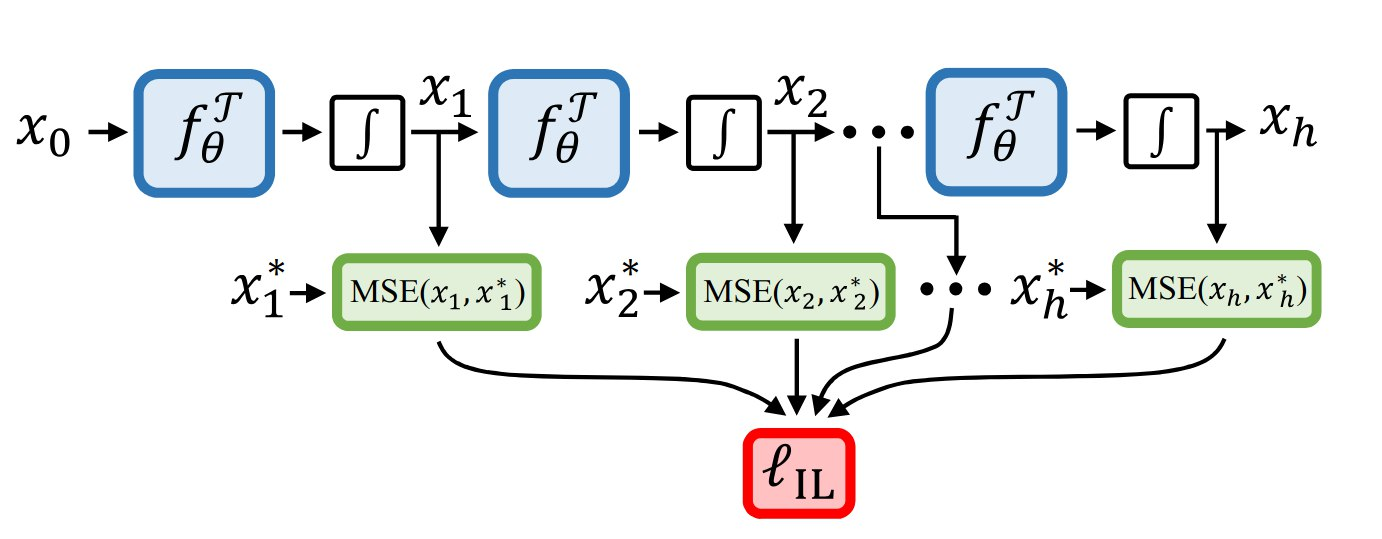
\includegraphics[width=\textwidth]{../report/assets/mlp_1.jpg} % replace with 
            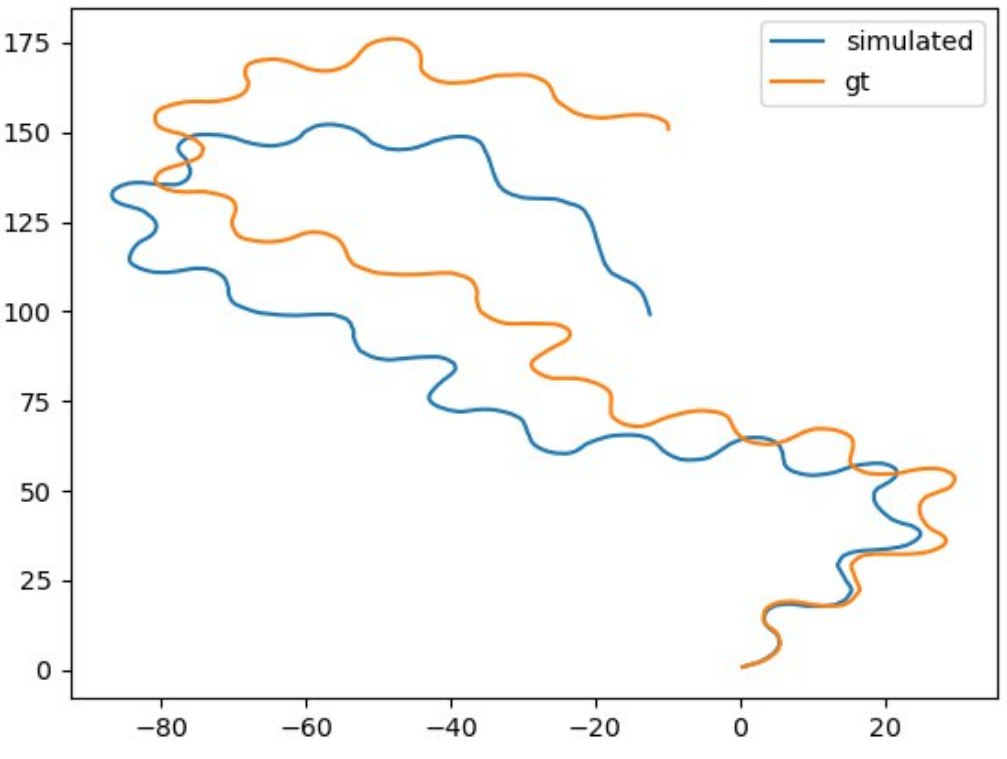
\includegraphics[width=\textwidth]{../report/assets/mlp_2.jpg} % replace with your second image file
            \footnotesize{Evolution Trajectory}
        \end{column}
    \end{columns}
\end{frame}

\section{Physical Informed Neural Networks}
\begin{frame}{PiNNs}
    \begin{columns}[T]
        % Right Column: Text and Equations
        \begin{column}{0.55\textwidth}
            Physical Informed Neural Networks (PiNNs) propose an alternative approach where the solution is approximated by a neural network that is trained not only on data but also by enforcing the underlying physical laws via the differential equations.
            \vspace{1em}
            \begin{align}
                \mathcal{L}_{\text{data}}(\theta) &= \frac{1}{N_u} \sum_{i=1}^{N_u} \left| u_{\theta}(\mathbf{x}_i, t_i) - u^{\text{obs}}_i \right|^2, \\
                \mathcal{L}_{\text{phys}}(\theta) &= \frac{1}{N_r} \sum_{j=1}^{N_r} \left| \mathcal{N}[u_{\theta}](\mathbf{x}_j, t_j) \right|^2,
            \end{align}
        \end{column}

        \begin{column}{0.4\textwidth}
            \centering
            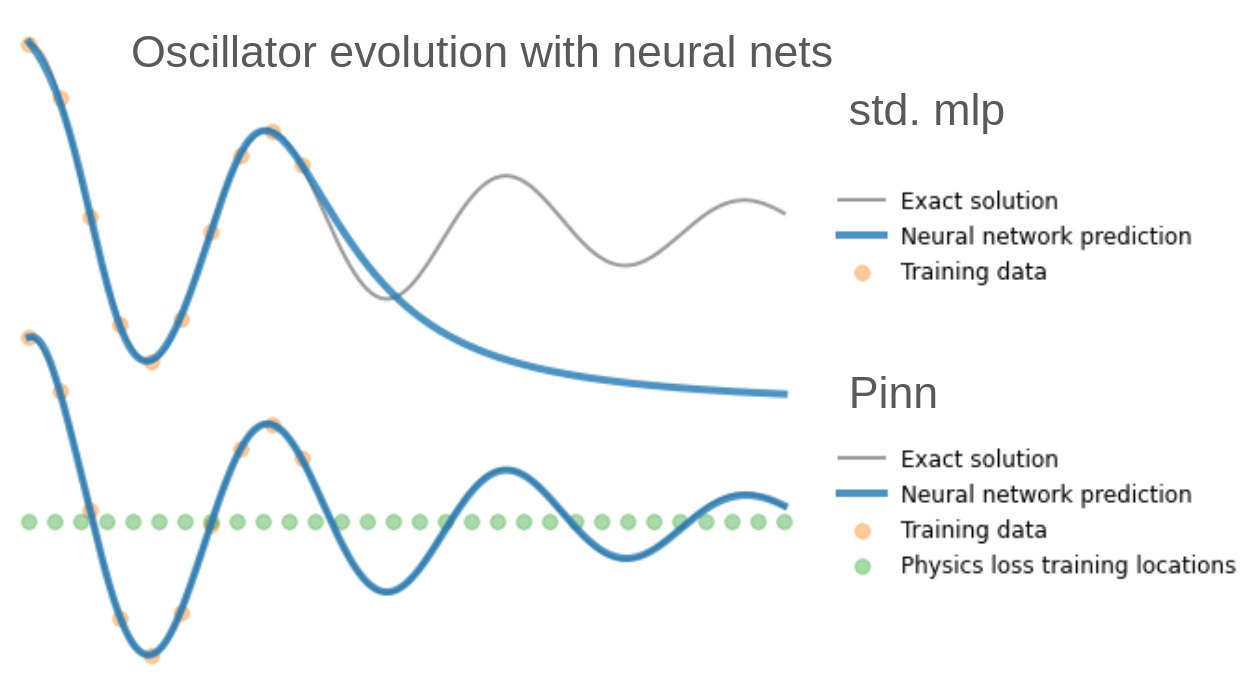
\includegraphics[width=\textwidth]{../report/assets/oscillator.jpg} % Replace with your image file
            \vspace{1ex}
            \footnotesize{PiNN vs Classical MLP}
            \\
            \textbf{Problems and Limitations}:
            \begin{itemize}
                \item Cannot handle control input 
                \item Fixed initial condition
            \end{itemize}
        \end{column}
        
    \end{columns}
\end{frame}
\begin{frame}{PiNN with Controls}
    \begin{columns}[T]
        % Right Column: Text and Equations
        \begin{column}{0.55\textwidth}
            The Pinn-C modifies the formulation of the pinn, by dividing the evolution into sub-transitions with constant input. The network takes as input $(x(0), \bar{u}, t)$. \\
            \vspace{1ex}
            \textbf{Pros}:
            \begin{itemize}
                \item it can handle larger time-steps with respect to the original formulation
                \item can accept arbitrary starting conditions
            \end{itemize}
            \textbf{Cons}:
            \begin{itemize}
                \item relies heavily on the dataset 
            \end{itemize}
        \end{column}

        \begin{column}{0.4\textwidth}
            \centering
            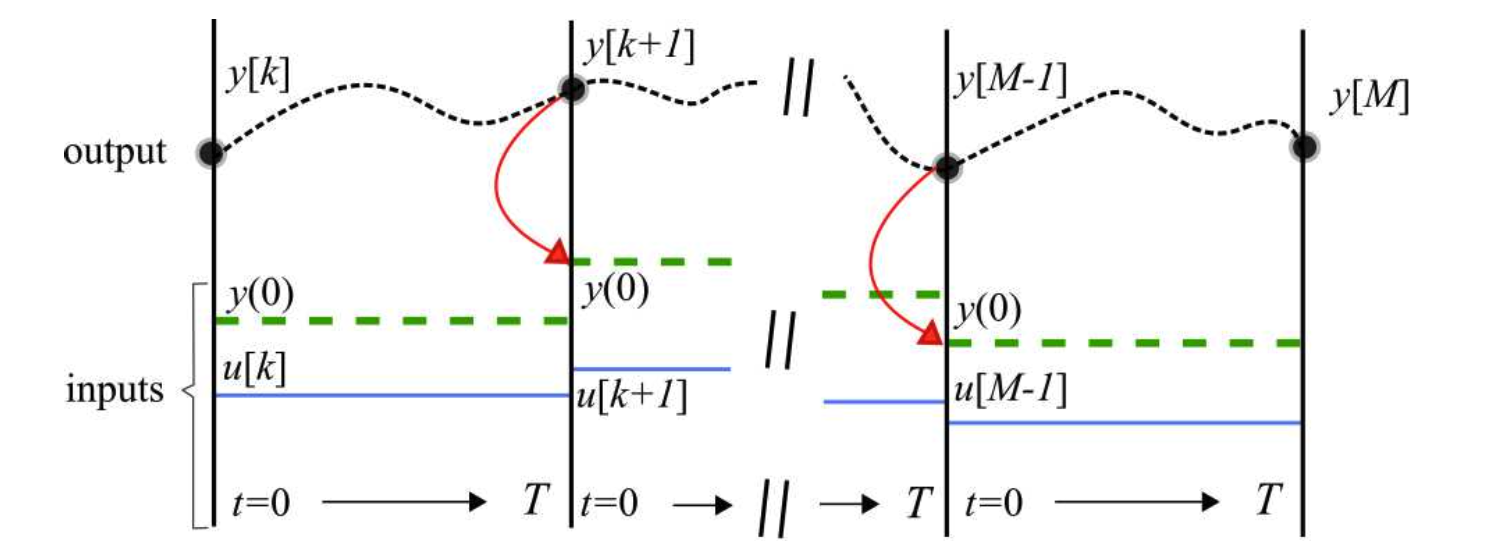
\includegraphics[width=\textwidth]{../report/assets/pinc_time.png} % Replace with your image file
            \vspace{1ex}
            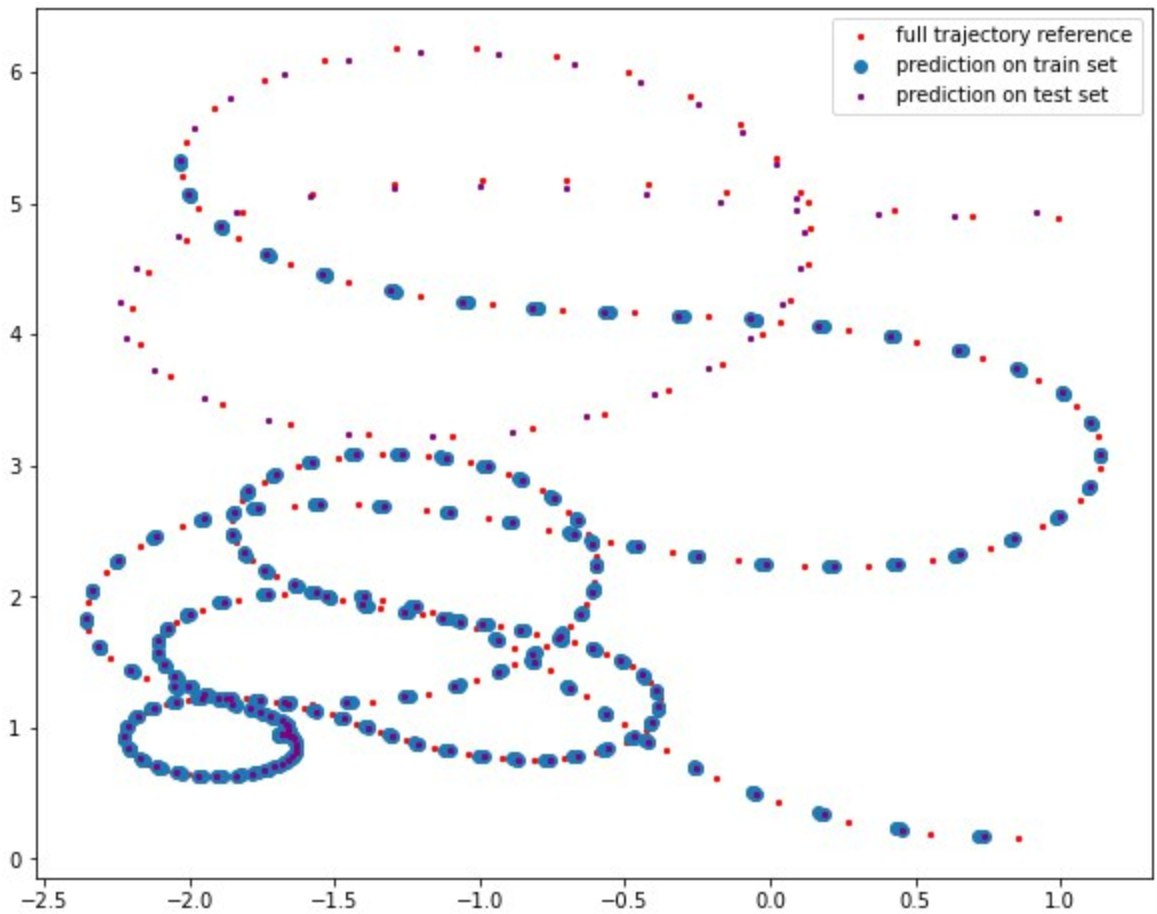
\includegraphics[width=0.9\textwidth]{../report/assets/pinnc_traj.jpg} % Replace
            \footnotesize{Trajectory with PiNN-C}
        \end{column}
        
    \end{columns}
\end{frame}
\section{Results and Problems Encountered}
\begin{frame}{Dataset Generation}
We have tried different strategies:
\begin{itemize}
    \item random velocity commands over the horizon
    \item random velocity commands constant over the horizon
\end{itemize}
The system has been integrated with Euler or Runge-Kutta 4.
\end{frame}

\begin{frame}{Drift Problem}
        \begin{columns}[T] % Align columns at the top
            % Left Column: Text
            \begin{column}{0.55\textwidth}
                After some training, we have tested our neural model along with the MPC with nice results (check video). However, we found that by having zero control inputs the network still moves the state somewhere else. We have tried to overcome this problem in some ways but with poor results:
                \begin{itemize}
                    \item Sample \(N\) points at the boundary during each epoch
                    \item Add a penalty term related to the boundary condition
                \end{itemize}
            \end{column}
            % Right Column: Image
            \begin{column}{0.40\textwidth}
                \centering
                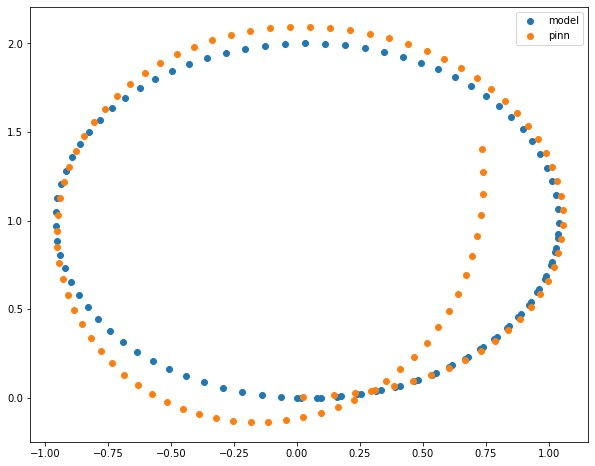
\includegraphics[width=\textwidth, keepaspectratio]{../report/assets/mlp_circle.jpg} % Replace with your image file
                \vspace{1ex}
                \footnotesize{PiNN-C vs Reference}
            \end{column}
        \end{columns}
    \end{frame}
\begin{frame}{Possible Local Minima}
    \begin{columns}[T] % Align columns at the top
        % Left Column: Text
        \begin{column}{0.55\textwidth}
            \vspace{1ex}
            During each training experiment, we have found that all losses behave correctly but they remain stuck at some points even with few iterations. Also in this case we have tried extensively hyperparameter tuning without any solution to the problem.
        \end{column}
        % Right Column: Image
        \begin{column}{0.40\textwidth}
            \centering
            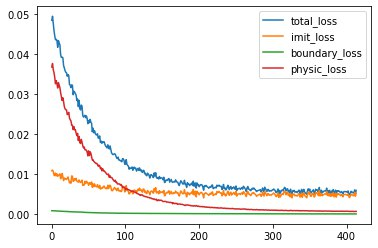
\includegraphics[width=\textwidth,keepaspectratio]{../report/assets/loss.jpg}
            \footnotesize{Loss Behavior}
        \end{column}
    \end{columns}
\end{frame}
% \backmatter add this later
\end{document}
